% answers.tex —— 1977 年·河北卷 · 参考答案与详细解析片段
% 由 tools/generate_projects.py 依来源总账自 1977/1977_数学真题_河北_试题.md + 1977/1977_数学真题_河北_解析正文.md + 1977/1977_数学真题_河北_答案要点.md 生成，勿手改（改源 MD 后重跑）


\begin{gktip}
固定源为 A3 单页题面，未附答案页；下列推导由编者独立完成，非官方标准答案。第 9 题是原卷附加题。
\end{gktip}

\begin{answer}
\gksolhead{1}{}

\textbf{题目}：

解答下列各题：

（1） 叙述函数的定义。

\Needspace{5\baselineskip}
（2） 求函数

\nopagebreak[4]
\[
y=1-\frac1{\sqrt{2-3x}}
\]

的定义域。

\Needspace{5\baselineskip}
（3） 计算：

\nopagebreak[4]
\[
\left[1-(0.5)^{-2}\right]\div\left(-\frac{27}{8}\right)^{\frac13}.
\]

（4） 计算：$\log_4 2$。

（5） 分解因式：$x^2y-2y^3$。

\Needspace{5\baselineskip}
（6） 计算：

\nopagebreak[4]
\[
\sin\frac{4\pi}{3}\cdot\cos\frac{25\pi}{6}\cdot\tan\left(-\frac{3\pi}{4}\right).
\]

\Needspace{4\baselineskip}
\textbf{解析}

\gksubpart{（1）}

函数是这样一种对应关系：对于给定的定义域中每一个自变量值，按照某种确定的对应法则，都有唯一确定的函数值与之对应。

\gksubpart{（2）}

根式在分母中，须有 $2-3x>0$，所以定义域为 $x<2/3$。

\gksubpart{（3）}

\nopagebreak[4]
\[
\left[1-(0.5)^{-2}\right]\div\left(-\frac{27}{8}\right)^{1/3}
=\left(1-4\right)\div(-3)=1.
\]

\gksubpart{（4）}

\nopagebreak[4]
\[
\log_4 2=\frac12.
\]

\gksubpart{（5）}

\nopagebreak[4]
\[
x^2y-2y^3=y(x^2-2y^2).
\]

\gksubpart{（6）}

\nopagebreak[4]
\[
\sin\frac{4\pi}{3}=-\frac{\sqrt3}{2},
\quad
\cos\frac{25\pi}{6}=\cos\frac\pi6=\frac{\sqrt3}{2},
\quad
\tan\left(-\frac{3\pi}{4}\right)=1.
\]

三者相乘得 $-3/4$。

\gkanswer{答案（1）：见解析版}

\gkanswer{答案（2）：$x<\dfrac23$。}

\gkanswer{答案（3）：$1$。}

\gkanswer{答案（4）：$\dfrac12$。}

\gkanswer{答案（5）：$y(x^2-2y^2)$。}

\gkanswer{答案（6）：$-\dfrac34$。}

\end{answer}
\begin{answer}
\gksolhead{2}{}

\textbf{题目}：

证明：如图，$AB$ 是圆 $O$ 的直径，$CB$ 是圆 $O$ 的切线，切点为 $B$，$OC$ 平行于弦 $AD$，求证：$DC$ 是圆 $O$ 的切线。
\nopagebreak[4]
\begin{center}% 1977 年河北卷第 2 题：直径、切线与平行弦
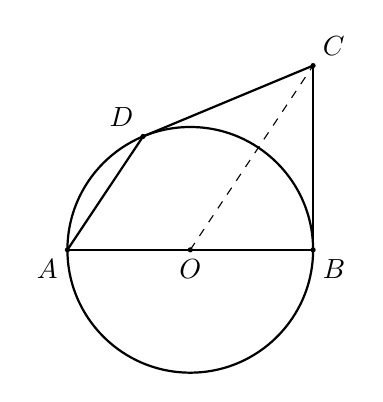
\begin{tikzpicture}[scale=0.78,>=stealth]
  \coordinate (O) at (0,0);
  \coordinate (A) at (-2,0);
  \coordinate (B) at (2,0);
  \coordinate (C) at (2,3);
  \coordinate (D) at (-0.769,1.846);
  \draw[thick] (O) circle (2);
  \draw[thick] (A)--(B);
  \draw[thick] (B)--(C);
  \draw[thick] (A)--(D);
  \draw[thick] (D)--(C);
  \draw[dashed] (O)--(C);
  \fill (O) circle (1.2pt) node[below] {$O$};
  \fill (A) circle (1.2pt) node[below left] {$A$};
  \fill (B) circle (1.2pt) node[below right] {$B$};
  \fill (C) circle (1.2pt) node[above right] {$C$};
  \fill (D) circle (1.2pt) node[above left] {$D$};
\end{tikzpicture}
\end{center}
\nopagebreak[4]
\Needspace{4\baselineskip}
\textbf{解析}

\Needspace{5\baselineskip}
设圆半径为 $R$。取坐标系使 $O=(0,0)$、$A=(-R,0)$、$B=(R,0)$，因 $CB$ 在 $B$ 点切圆，设 $C=(R,t)$。由 $OC\parallel AD$，弦 $AD$ 的方向向量可取 $(R,t)$，故令

\nopagebreak[4]
\[
D=A+\lambda(R,t).
\]

\Needspace{5\baselineskip}
将 $D$ 在圆 $x^2+y^2=R^2$ 上代入，除去 $D=A$ 的根，得到

\nopagebreak[4]
\[
\lambda=\frac{2R^2}{R^2+t^2}.
\]

\Needspace{5\baselineskip}
于是

\nopagebreak[4]
\[
\overrightarrow{OD}\cdot\overrightarrow{DC}=0,
\]

即 $OD\perp DC$。因此 $DC$ 是圆 $O$ 在 $D$ 点的切线。

\gkanswer{答案：见解析版}

\end{answer}
\begin{answer}
\gksolhead{3}{}

\textbf{题目}：

\Needspace{5\baselineskip}
证明：

\nopagebreak[4]
\[
\frac{\sin2\alpha+1}{1+\cos2\alpha+\sin2\alpha}=\frac12\tan\alpha+\frac12.
\]

\Needspace{4\baselineskip}
\textbf{解析}

\Needspace{5\baselineskip}
用 $\sin2\alpha=2\sin\alpha\cos\alpha$、$1+\cos2\alpha=2\cos^2\alpha$，原式左端为

\nopagebreak[4]
\[
\frac{1+2\sin\alpha\cos\alpha}{2\cos^2\alpha+2\sin\alpha\cos\alpha}
=\frac{1+\sin\alpha}{2\cos\alpha}
=\frac12\tan\alpha+\frac12,
\]

在原式有意义的范围内等式成立。

\gkanswer{答案：见解析版}

\end{answer}
\begin{answer}
\gksolhead{4}{}

\textbf{题目}：

已知 $2\lg x+\lg2=\lg(x+6)$，求 $x$。

\Needspace{4\baselineskip}
\textbf{解析}

\Needspace{5\baselineskip}
由定义域 $x>0$，合并对数得

\nopagebreak[4]
\[
\lg(2x^2)=\lg(x+6),
\]

\Needspace{5\baselineskip}
所以 $2x^2=x+6$，即

\nopagebreak[4]
\[
2x^2-x-6=0,
\qquad
(2x+3)(x-2)=0.
\]

结合 $x>0$，得 $x=2$。

\gkanswer{答案：$x=2$。}

\end{answer}
\begin{answer}
\gksolhead{5}{}

\textbf{题目}：

某生产队要建立一个形状是直角梯形的苗圃，其两邻边借用夹角为 $135^\circ$ 的两面墙，另外两边是总长为 $30$ 米的篱笆（如图，$AD$ 和 $DC$ 为墙），问篱笆的两边各多长时，苗圃的面积最大？最大面积是多少？
\nopagebreak[4]
\begin{center}% 1977 年河北卷第 5 题：两面墙与篱笆围成的直角梯形
\begin{tikzpicture}[scale=0.78]
  \coordinate (A) at (0,0);
  \coordinate (B) at (5.2,0);
  \coordinate (C) at (5.2,2.6);
  \coordinate (D) at (2.6,2.6);
  \draw[thick] (A)--(B)--(C)--(D)--cycle;
  \draw[very thick] (A)--(D) node[midway,left] {墙};
  \draw[very thick] (D)--(C) node[midway,above] {墙};
  \node[below left] at (A) {$A$};
  \node[below right] at (B) {$B$};
  \node[above right] at (C) {$C$};
  \node[above left] at (D) {$D$};
  \node[below] at (2.6,0) {篱笆};
  \node[right] at (5.2,1.3) {篱笆};
\end{tikzpicture}
\end{center}
\nopagebreak[4]
\Needspace{4\baselineskip}
\textbf{解析}

\Needspace{5\baselineskip}
设篱笆的水平边 $AB=x$ 米，竖直边 $BC=y$ 米，则 $x+y=30$。由墙的夹角为 $135^\circ$，图示直角梯形的上底为 $x-y$，高为 $y$，面积为

\nopagebreak[4]
\[
S=\frac{x+(x-y)}2y=xy-\frac12y^2.
\]

\Needspace{5\baselineskip}
代入 $x=30-y$：

\nopagebreak[4]
\[
S=30y-\frac32y^2=150-\frac32(y-10)^2.
\]

故 $y=10$、$x=20$ 时面积最大，最大值为 $150\ \mathrm{m^2}$。

\gkanswer{答案：篱笆两边分别为 $20$ 米、$10$ 米；最大面积为 $150\ \mathrm{m^2}$。}

\end{answer}
\begin{answer}
\gksolhead{6}{}

\textbf{题目}：

工人师傅要用铁皮做一个上大下小的正四棱台形容器（上面开口），使其容积为 $208$ 立方米，高为 $4$ 分米，上口边长与下底面边长的比为 $5:2$，做这样的容器需要多少平方米的铁皮？（不计容器的厚度和加工余量，不要求写出已知、求解，直接求解并画图即可。）

\Needspace{4\baselineskip}
\textbf{解析}

\Needspace{5\baselineskip}
严格按源卷单位计算。设下底面正方形边长为 $s$ 米，则上底面边长为 $5s/2$ 米，高 $4$ 分米即 $2/5$ 米。棱台体积为

\nopagebreak[4]
\[
208=\frac{2/5}{3}\left(s^2+\frac{25s^2}{4}+\frac{5s^2}{2}\right)=\frac{13}{10}s^2,
\]

\Needspace{5\baselineskip}
所以 $s^2=160$，下底边长 $s=4\sqrt{10}$ 米，上口边长为 $10\sqrt{10}$ 米。侧面梯形的斜高为

\nopagebreak[4]
\[
\ell=\sqrt{\left(\frac25\right)^2+(3\sqrt{10})^2}=\frac{\sqrt{2254}}5.
\]

\Needspace{5\baselineskip}
容器上面开口，铁皮面积为底面积加四个侧面面积：

\nopagebreak[4]
\[
\begin{aligned}
S&=160+4\cdot\frac{4\sqrt{10}+10\sqrt{10}}2\cdot\frac{\sqrt{2254}}5\\
&=160+\frac{56\sqrt{5635}}5\ \mathrm{m^2}.
\end{aligned}
\]

\gkanswer{答案：严格按原卷“208 立方米、4 分米”计算，$160+\dfrac{56\sqrt{5635}}5\ \mathrm{m^2}$。}

\end{answer}
\begin{answer}
\gksolhead{7}{}

\textbf{题目}：

\Needspace{5\baselineskip}
如图，$MN$ 为圆的直径，$P\text{、}C$ 为圆上两点，连 $PM\text{、}PN$，过 $C$ 作 $MN$ 的垂线与 $MN\text{、}MP$ 和 $NP$ 的延长线依次相交于 $A\text{、}B\text{、}D$，求证：

\nopagebreak[4]
\[
AC^2=AB\cdot AD.
\]
\nopagebreak[4]
\begin{center}% 1977 年河北卷第 7 题：圆内直径与外部相交线
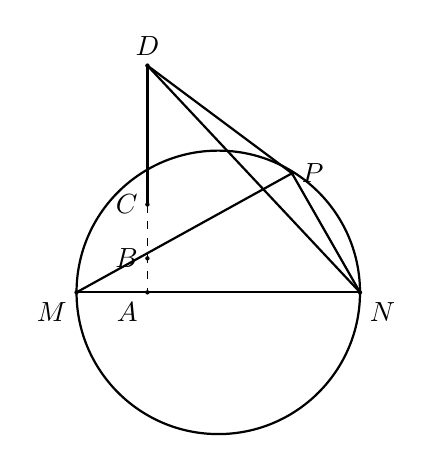
\begin{tikzpicture}[scale=0.72,>=stealth]
  \coordinate (M) at (0,0);
  \coordinate (N) at (5,0);
  \coordinate (O) at (2.5,0);
  \coordinate (P) at (3.8,2.1);
  \coordinate (C) at (1.25,1.55);
  \coordinate (D) at (1.25,4.0);
  \coordinate (A) at (1.25,0);
  \coordinate (B) at (1.25,0.6);
  \draw[thick] (M) arc (180:540:2.5);
  \draw[thick] (M)--(N);
  \draw[thick] (P)--(M) (P)--(N);
  \draw[thick] (D)--(P);
  \draw[thick] (D)--(C);
  \draw[thick] (D)--(N);
  \draw[dashed] (C)--(A);
  \fill (M) circle (1.1pt) node[below left] {$M$};
  \fill (N) circle (1.1pt) node[below right] {$N$};
  \fill (P) circle (1.1pt) node[right] {$P$};
  \fill (C) circle (1.1pt) node[left] {$C$};
  \fill (D) circle (1.1pt) node[above] {$D$};
  \fill (A) circle (1.1pt) node[below left] {$A$};
  \fill (B) circle (1.1pt) node[left] {$B$};
\end{tikzpicture}
\end{center}
\nopagebreak[4]
\Needspace{4\baselineskip}
\textbf{解析}

\Needspace{5\baselineskip}
由于 $CA\perp MN$，且 $MN$ 是直径，故 $\angle MCN=90^\circ$。又 $C\text{、}B\text{、}D$ 共线，$A\text{、}C$ 与 $MN$ 垂直。由相交弦与相似三角形关系，$\triangle ACB\sim\triangle ADC$：其中 $\angle CAB=\angle CAD$（同为弦方向与 $MN$ 的夹角），且直线 $BD$ 与 $AC$ 的对应角相等。因此

\nopagebreak[4]
\[
\frac{AC}{AB}=\frac{AD}{AC},
\]

即 $AC^2=AB\cdot AD$。

\gkanswer{答案：见解析版}

\end{answer}
\begin{answer}
\gksolhead{8}{}

\textbf{题目}：

下列两题选做一题。

【甲】已知椭圆短轴长为 $2$，中心与抛物线 $y^2=4x$ 的顶点重合，椭圆的一个焦点恰是此抛物线的焦点，求椭圆方程及其长轴的长。

【乙】已知菱形的一对内角各为 $60^\circ$，边长为 $4$，以菱形对角线所在的直线为坐标轴建立直角坐标系，以菱形 $60^\circ$ 角的两个顶点为焦点，并且过菱形的另外两个顶点作椭圆，求椭圆方程。

\begin{gktip}
\Needspace{0.25\textheight}
\textbf{附加题}
\end{gktip}

\textbf{附加题 9．} 将函数 $f(x)=\mathrm e^x$ 展开为 $x$ 的幂级数，并求出收敛区间。（$\mathrm e=2.718$ 为自然对数的底数。）

\Needspace{4\baselineskip}
\textbf{解析}

\Needspace{5\baselineskip}
【甲】抛物线 $y^2=4x$ 的焦点为 $(1,0)$，所以椭圆半焦距 $c=1$；短轴长为 $2$，故 $b=1$。椭圆中心为原点，$a^2=b^2+c^2=2$，从而

\nopagebreak[4]
\[
\frac{x^2}{2}+y^2=1,
\]

长轴长为 $2a=2\sqrt2$。

\Needspace{5\baselineskip}
【乙】取菱形 $60^\circ$ 角的两个顶点为焦点。菱形边长为 $4$，长对角线为 $4\sqrt3$，短对角线为 $4$；以长对角线为 $x$ 轴时，焦点为 $(\pm2\sqrt3,0)$，另外两个顶点为 $(0,\pm2)$。椭圆半焦距 $c=2\sqrt3$、短半轴 $b=2$，故 $a^2=b^2+c^2=16$，方程为

\nopagebreak[4]
\[
\frac{x^2}{16}+\frac{y^2}{4}=1.
\]

\gksubpart{附加题 9}

\Needspace{4\baselineskip}
\textbf{解析}

\Needspace{5\baselineskip}
指数函数的 Maclaurin 展开为

\nopagebreak[4]
\[
\mathrm e^x=1+x+\frac{x^2}{2!}+\frac{x^3}{3!}+\cdots+\frac{x^n}{n!}+\cdots.
\]

\Needspace{5\baselineskip}
由比值判别法，任意 $x$ 下级数均收敛，因此收敛区间为

\nopagebreak[4]
\[
(-\infty,+\infty).
\]

\gkanswer{答案：选作【甲】时，椭圆方程为 $\dfrac{x^2}{2}+y^2=1$，长轴长为 $2\sqrt2$；选作【乙】时，椭圆方程为 $\dfrac{x^2}{16}+\dfrac{y^2}{4}=1$。}

\end{answer}